\documentclass[12pt]{article}
\usepackage[english]{babel}
\usepackage{hyperref}
\usepackage{makeidx}
\usepackage{chngcntr}
\usepackage{pgfplots}
\usepackage[utf8]{inputenc}
\usepackage[acronym]{glossaries}
\usepackage[a4paper, inner=1.5cm, outer=3cm, top=2cm,bottom=3cm, bindingoffset=1cm]{geometry}

\counterwithin*{section}{part}
\usepackage{tikz}
\usetikzlibrary{arrows.meta}
\tikzset{%
  >={Latex[width=2mm,length=2mm]},
  % Specifications for style of nodes:
            base/.style = {rectangle, rounded corners, draw=black,
                           minimum width=4cm, minimum height=1cm,
                           text centered, font=\sffamily},
  activityStarts/.style = {base, fill=blue!30},
       startstop/.style = {base, fill=red!30},
    activityRuns/.style = {base, fill=green!30},
         process/.style = {base, minimum width=2.5cm, fill=orange!15,
                           font=\ttfamily},
}
\begin{document}
\begin{titlepage}
    \begin{center}
        \vspace*{1cm} 
        \Huge
        \textbf{Comparative approaches for classification of diabetes mellitus data.} 
        \vspace{0.5cm}
        \normalsize
        \vspace{0cm}
        \\
        Study of machine learning algorithms and application on the Pima Indians Diabetes Dataset.
 
        \vspace{1.5cm}
 
        \textbf{Alexander Roque Rodrigues}
 
        \vfill
 
        A dissertation presented for the degree of\\
        Bachelor in Computer Science
 
        \vspace{0.8cm}
  
        \Large
        Department of Computer Science\\        
        Smt. Parvatibai Chowgule College of Arts and Science\\
        India\\
        18 August 2019
 
    \end{center}
\end{titlepage}
\Huge
\newpage
\huge
\textbf{Acknowledgements}
\normalsize
\newpage
\tableofcontents
\newpage
\part{Background}
Data is everywhere. International initiatives coupled with global disruptive innovation are the leading causes for pushing datafincation forward.

\textbf{Datafication refers to the modern-day trend of digitalizing (or datafying) every aspect of life.}

This data creation is enabling the transformation of data into new and potentially valuable forms. Entire municipalities are being incentivized to become smarter. In the not too
distant future, our towns and cities will collect thousands of variables in
real time to optimize, maintain, and enhance the quality of life for entire
populations. One would reasonably expect that as well as managing traffic,
traffic lights may also collect other data such as air quality, visibility, and
speed of traffic. As a result of big data from connected devices, embedded
sensors, and the IoT, there is a global need for the analysis, interpretation,
and visualization of data.

\newpage
\part{Need for Research}

\section{A Case Study}
% source
\iffalse https://www.courant.com/news/connecticut/hc-xpm-2001-09-18-0109180410-story.html \fi

PIMA INDIANS: A CASE STUDY
GREG MORAGO; Courant Staff Writer
THE HARTFORD COURANT

It's in the blood. The blood of ancestors that carries a time bomb. The blood of my mother, both my grandmothers, my sister and dozens of relatives bound by an inherited disease.

It's in my blood, too -- a genetic predisposition to obesity, which is a major risk factor for diabetes. Diabetes has marked generations of my family and my tribe, the Pima Indians of southern Arizona. We Pimas -- cruelly targeted by a genetic quirk that has caused us to have the highest rate of diabetes in the world -- have long lived with the kidney disease, blindness and amputations that attend diabetes. And, of course, the death.

For decades, researchers have focused on our tribe to understand why the Pimas are at such an alarmingly high risk of getting diabetes.

With the help of Pima volunteers, scientists have learned that diabetes develops when a person's body doesn't use insulin effectively. Volunteers from our tribe continue to help support research not unlike the recent clinical trials that linked lifestyle changes to preventing diabetes. The very people living through, and dying from, diabetes have been in the forefront of diabetes prevention -- willing subjects for scientists studying a disease that is blossoming into a health epidemic.

I'm proud of my people. People like my aunt, Viola Johnson, head of health services on our reservation, who has worked with hundreds of researchers who have descended on our tribe to learn more about the disease. People like friends and relatives on our reservation who have been poked, prodded, weighed and measured in an effort not only to stave off health complications of their own disease but to help others who might get diabetes.

Then again, the Pimas -- who have lived in the Sonoran Desert near the Gila River for at least 2,000 years -- have always been helpful. They were trusted scouts for the U.S. Cavalry. Expert farmers, they shared their bounty with travelers and neighboring tribes long before we had reservations. Today, they are sharing the knowledge of living with diabetes in order to prevent it.

And yet, despite all we know about diabetes, we continue to court disaster. Inactivity and bad diet continue to deliver Pimas to the disease. I am a glaring example: an overweight, out-of-shape smoker who wines and dines recklessly. I am the perfect candidate for adult-onset diabetes. Although my mother constantly asks that I be tested, I have yet to let a doctor draw blood. As far as I know, I don't have diabetes, but I'm constantly on the watch for the warning signs -- the genetic smoke signals of my ancestors.

I have many inducements to be more careful. There's my grandmother, who lost toes on both feet last year after an infection. There's my mother, who pricks her fingers every day to test her blood sugar levels. There's my younger sister, who last year got diabetes and whose teenage son only recently learned he's borderline diabetic.

At least a dozen of my childhood friends are already dead. I've watched people who were overweight waste away. My uncle is on dialysis because diabetes has wrecked his kidneys.

But after years of attempting diets and making vows to get more exercise, I remain overweight -- the highest risk factor for diabetes. One-half of Pima adults have diabetes and 95 percent of those with diabetes are overweight.

Why are so many Pimas overweight? In the '60s, the "thrifty gene" theory helped explain. For thousands of years the Pimas, who relied on farming, hunting and fishing for food, experienced alternating periods of feast and famine. To adapt to these extreme changes in caloric needs, the Pimas developed a thrifty gene that allowed them to store fat in times of plenty in order to survive in times of famine. The gene was helpful as long as there were periods of famine. But when the Pimas adopted a Western lifestyle -- a higher-fat diet and physical inactivity -- the gene began to work against them.

Scientists believe the gene that protected Pimas from starvation now also contributes to retaining unhealthy amounts of fat. Scientists studying Pimas have determined that diabetes runs in families, along with insulin resistance and obesity. In other words, diabetes, for Pimas, is an inherited disease.

Today, our tribe prefers to see the positive side of living with the disease. Casino revenue pouring into our reservation is paying for wellness centers that promote exercise and health care education. It has already paid for a new hospital and more doctors not only treating Pimas but members of far-flung tribes without the medical care and facilities we enjoy.

It has paid for sophisticated treatment off the reservation, as well.

And maybe, if I'm not careful, it will end up paying for my diabetic health care. I hope not.

Despite the many tragedies, optimism abounds in the Pima community of the Gila River. We remain hopeful that the findings of recent, ongoing and new studies bring us all closer to preventing, maybe curing, diabetes. Hopeful that one day our proud blood won't so easily betray us.

\newpage
\section{Identifying Groups prone to Diabetes}
% source
\iffalse https://www.ncbi.nlm.nih.gov/pmc/articles/PMC4418458/ \fi
\subsection{Introduction}
The Pima Indians of Arizona and Mexico have contributed to numerous scientific gains through their willingness to participate in the research process. Their involvement has led to significant findings with regard to the epidemiology, physiology, clinical assessment, and genetics of both type 2 diabetes and obesity. Longitudinal investigations, starting in 1965, have involved study participants living on the Gila River Reservation outside Phoenix, Arizona and, since 1991, the residents of the community of Maycoba, Mexico.

The purpose of this review is broadly to summarize the contributions to our current knowledge resulting from the participation of the Pimas in both countries. It starts with the original documentation of the epidemic of diabetes and obesity among the Pimas of Arizona and proceeds to the developing concerns for their genetically-related counterparts in Mexico.

\subsection{History}
The O'odham (Arizona), O'ob also Pima Bajo (Mexico) [1], or Pima in general, are descendants of the ancient Hohokam, who have inhabited the Sonoran desert and Sierra Madre regions for centuries [2]. About 300 B.C. the Hohokam moved into the Gila River valley, at that time still Mexican territory [3]. After the United States acquired parts of northern Mexico in the 1853 Gadsden Purchase, the O'odham and the Pima Bajo became further separated and, ultimately, had little future contact. In 1959 a Pima reservation in Arizona was created and the majority of Arizona Pima continue to reside there [2].

The Pimas of Arizona adapted to their desert homeland by directing water through an elaborate system of irrigation canals to support subsistence agriculture; they grew corn, beans, squash and cotton [4]. Sadly, around 1900 the increased population of white settlers to the north led to the eventual diversion of the water that supported the Pimas' way of life [5].

The forced curtailment of farming led to significant impacts on their food intake, physical activity and their economy [6]. Their life changed from farming sustained though physical labor to one of food scarcity and little labor. Famine, rarely experienced in the past, became chronic. As a result, this time period marked the end of a lifestyle to which the Pima were well-adapted and transitioned to a lifestyle for which they were poorly adapted. Their low-fat, high-carbohydrate diet changed to one that ultimately derived more than forty percent of its energy from fat [7]. At the same time the demand for physical labor subsided.

The timing of this significant change in lifestyle and livelihood coincides with the development of diabetes among the Arizona Pimas. At the turn of the nineteenth century, Hrdlicka recorded one case on the Gila River Reservation [8]. In 1937, Joslin documented twenty-one persons with diabetes there and concluded that the presence of diabetes among the Pimas was similar to that of the general U.S. population [9]. By the 1950's, however, the prevalence had increased ten-fold [10], and a study initiated in 1965 documented in the Arizona Pima Indians the highest prevalence of diabetes ever recorded [11].

The onset of this epidemic stimulated a longitudinal study initiated at the Sacaton Service Unit of the Indian Health Services. Residents of the Gila River Indian Reservation, regardless of health status, who were of at least half Pima ancestry and age five and older, were invited to participate. Each volunteer was examined approximately every two years. The examinations included a medical history, physical examination, medical record review and oral glucose tolerance test [12].

Using ten years of this longitudinal data (periodic glucose tolerance testing and medical record reviews) a comparison of diabetes prevalence and incidence was assembled between the Arizona Pimas and the predominantly White population of Rochester, Minnesota. The results indicated that the Pima had a nineteen-fold greater incidence of diabetes than the sample population in Rochester [12]. Although it was already known that Native heritage is associated with higher diabetes prevalence [13], the situation with the Pima was unique.

The frequency of type 2 diabetes has continued to increase. By 1970, the prevalence of type 2 diabetes was about forty percent among Pimas age thirty-five and older, and currently affects about half of all Pimas over age thirty-five [14]. By the mid-1970s, the Pima were also more obese than similarly aged Caucasians [5]. Studies supporting the familial nature of diabetes and obesity among the Pimas indicated a clear genetic component to these disorders [5]. But how would a propensity for the development of type 2 diabetes and obesity accommodate the “survival of the fittest” explanation of genetic selection?

\subsection{Energy Expenditure}
By comparing the physical activity level of 40 (17 female and 23 males) Mexican Pima Indians with 40 age- and sex-matched Pimas from the Gila River Indian Community (Arizona), the potential protective role of environment and physical activity against obesity was measured [21]. Total energy expenditure (TEE), measured with doubly-labeled water, was used to determine physical activity levels. Resting metabolic rate (RMR) was also calculated to determine physical activity levels (PAL). Four PAL indices were calculated: TEE to RMR ratio, TEE adjusted for RMR using linear regression analysis, activity energy expenditure (AEE) adjusted for body weight, also using regression analysis, and a translated activity questionnaire including occupational and leisure activities [22].

The PAL, TEE adjusted for RMR, and AEE adjusted for body weight results all showed that physical activity was higher in Mexican Pima when compared to Arizona Pima. The activity questionnaire indicated that Mexican Pima spend more time on occupational activities than Arizona Pima. Therefore we concluded that physical activity plays a significant role in the prevention of obesity in genetically susceptible populations [21].

\subsection{Leptin}
Leptin is an important signal for the regulation of energy stores. The impact of environment on leptin concentration was examined by comparing Mexican Pima Indians (N=224) still living a traditional lifestyle with Arizona Pimas (N=418) living a more modern lifestyle [23]. We hypothesized that the absolute value of leptin would be lower in Mexican Pimas because of their lower percent body fat, but that leptin could be further influenced by their lifestyle, independent of body composition. Indeed, leptin concentration was strongly correlated with percent fat in both groups. Among the Arizona Pimas, independent of percent fat, research participants with type 2 diabetes had lower leptin concentrations than non-diabetic participants. Among non-diabetic individuals, Mexican Pimas had lower absolute leptin concentrations than Arizona Pimas, but higher leptin concentrations after adjustment for percent body fat, waist circumference, age and sex. In a subset of seventy pairs of subjects matched for sex and percent body fat, leptin concentrations were significantly higher in Mexican Pimas than their Arizona counterparts. These results suggested that independent of body composition, leptin concentration may be increased by environmental factors, such as diet and physical activity [23].

Another aspect of the “thrifty gene” hypothesis was tested with the cooperation of the two Mexican populations in Maycoba (Pima and non-Pima) by examining leptin concentrations and resting metabolic rate [24]. Whereas the thrifty gene may be wreaking havoc with the health of the Pimas in Arizona it may continue to play a beneficial role in the Mexican Pimas. Due to their remote environment, with limited access to amenities associated with modernization, the Mexican Pimas remain lean and they potentially manifest physiologic mechanisms promoting the metabolic efficiency associated with the thrifty genotype. Because the non-Pima Mexicans living in the same village are of predominantly European heritage, and therefore not considered to possess the thrifty genotype, it is less likely they would express these metabolic characteristics. Therefore, we hypothesized that if low plasma leptin and low metabolic rate are expressions of the thrifty gene, this difference would be more apparent in the Pima versus non-Pima populations living in the same environment. To test this hypothesis non-diabetic Mexican Pima Indians (N=208) were compared with non-diabetic non-Pima Mexicans (N=183) living in the same environment. Leptin concentrations were strongly correlated with percentage body fat in both groups, yet there appeared no significant difference in plasma leptin concentrations between the groups. Similarly, no significant different was shown in resting metabolic rate between groups. Therefore, these results did not support the hypothesis that hypoleptinemia, a low resting metabolic rate, or both hypoleptinemia and low resting metabolic, are expressions of the thrifty genotype.

\subsection{Insulin resistance}
Insulin resistance has been identified as a major risk factor in the pathogenesis of type 2 diabetes and has been thoroughly studied in the Arizona Pimas [25]. Given the lifestyle differences between the Mexican Pimas and their genetically-related counterparts in Arizona, we hypothesized that the Mexican group would be less insulin resistant. The study population included 194 Mexican Pima Indians and 449 Arizona Pimas, all of whom had normal glucose tolerance. Results showed that Mexican Pimas are less insulin resistant than Arizona Pimas, even after adjusting for age, sex and obesity [26]. These results emphasize the importance of lifestyle as a protective factor in the development of type 2 diabetes.

\subsection{Kidney disease}
Another aspect of type 2 diabetes examination based on data obtained from Arizona and Mexican Pima Indians was the association between diabetes and kidney disease. The Arizona Pimas have an extraordinarily high rate of kidney disease attributable to diabetes and kidney failure is a leading cause of death. More than half of Arizona Pimas with type 2 diabetes develop clinical proteinuria within twenty years of diagnosis. Once proteinuria develops, an irreversible deterioration of kidney function often ensues that leads to end-stage renal failure [27].

Since both diabetes and kidney disease have genetic and environmental determinates, measures of urine albumin and creatinine concentrations were made from samples obtained in the Maycoba-wide survey of diabetes and obesity. Ultimately, the prevalence of elevated urinary albumin excretion proved higher in Pima Indians with diabetes than in those without, regardless of whether they lived in Arizona or Mexico. Therefore, although diabetes has major environmental determinants, once diabetes develops, kidney disease will follow in populations susceptible to this complication [28].

\subsection{Environmental change}
The original series of studies concluded that even in populations genetically prone to type 2 diabetes and obesity, their development is determined mostly by environmental circumstances. The environment is never static, however. Over the years, the environmental circumstances of the Mexican Pimas and non-Pimas have changed. A partial electrical supply became available and allowed access to television, cars were more readily available along with mechanized devices to alter energy expenditure, and small grocery stores dotted the main road.

In light of these changes, a fifteen-year follow up study began in 2010 to identify changes in the Maycoba environment and determine whether these changes were associated with differences in diabetes and obesity prevalence. Measurements made in the 1995 study were replicated as closely as possible, including a medical history, biochemical and anthropometric measures, physical activity and dietary assessments [17]. Early in the study, a repeat census was conducted to determine the current demographic profile of the study area. All women and men over twenty years old, regardless of ethnicity, were invited to participate. The population increased minimally between 1995 and 2010, and 94\% of the individuals who took part in the 1995 study participated in again 2010.

Some results were predictable while others were surprising. Over the fifteen-year timeframe, the age-sex-adjusted diabetes prevalence was unchanged in Mexican Pima men yet it increased in non-Pima men. Prevalence of type 2 diabetes tended to increase in both Mexican Pima women and non-Pima women. Body mass index increased in all groups [29]. Therefore, we concluded that the transition from a traditional to modernized lifestyle is associated with diabetes and obesity, regardless of genetic predisposition.

These results made it imperative to identify the details of modernization that preceded the increased prevalence of type 2 diabetes and obesity in Maycoba. Novel assessments were put into play to document environmental change. These included a qualitative assessment on gardening and cultivation perceptions and patterns, a land-use, land-cover analysis, and an examination of the food environment (acquisition, behavior, and availability).

The role of family gardens was examined with regard to their impact on food consumption and physical labor [30]. Qualitative methods--interviews, two focus groups, and a household survey--were employed to explore changes in gardening and cultivation practices over the fifteen-year span between the two studies. The main findings indicated that home gardens and large plots for cultivation continue to contribute significantly to the food supply, although the majority of Pimas believed that food from cultivation had declined along with the amount of work families and children put into gardening. This decrease was partially attributed to climate change (e.g., lower rainfall) and increased access to processed foods. These findings suggested that change has occurred, but not as dramatic as originally presumed. The physical activity linked to cultivation may continue as an important factor in weight control and thereby, the prevention of diabetes [30].

The ecological environment linked to potential changes in lifestyle was also examined through impacts to the landscape [31]. A land-use and land-cover analysis was conducted of the Maycoba geographic area using aerial photos from 1994 and satellite images from 2007. This analysis was intended to examine transitions in the landscape, particularly from agricultural land-use to urbanized land-use, consistent with a decreased demand for physical activity. The findings indicated that the land-cover of the study area is mainly mixed vegetation and dense tree cover, a small percent of impermeable area, indicative of a rural environment. The land-use findings indicate a decrease or consistency in agricultural or ranching land and a decrease in farmland as seen through reforestation and re-vegetation in the Maycoba region. To examine lifestyle change three variables served as proxies: urban development, dwelling-unit density, and road network changes. The most notable changes were found in the town of Maycoba where urbanization, and the number and density of dwelling units increased. Only minor changes in the road network had occurred, as the interstate highway traversing the study area had opened prior to the start of the 1995 study. During the fifteen-year span the land-use and land-cover and proxy measures for lifestyle change in the Maycoba region have changed in a manner consistent with decreased physical activity [31].

Changes in the food environment were also examined [32]. Food acquisition was investigated through a representative household survey, two focus group discussions, and participant observation. The food retail environment changes were determined by auditing seven stores in the area. Findings showed that the food environment has changed dramatically in certain respects, with an increase in the presence of retail food stores, a wider selection of processed foods, an increase in perishable foods due the introduction of regular electricity, and the prominent placement of certain packaged foods. In juxtaposition, traditional subsistence-based activities such as cultivating, ranching, hunting, and gathering, remain important to daily life. Although there had been a noticeable decline in subsistence activities, a traditional lifestyle had persisted in the Maycoba region at the time of the follow-up study.

\subsection{Conclusion}
The Pimas of Arizona and Mexico have played a crucial role in scientific advances in type 2 diabetes and obesity. In conjunction, the two groups have provided a unique opportunity to understand the independent roles of genes versus environment because they are genetically-related populations living in dramatically different environments yet presenting with significant differences in diabetes and obesity prevalence. These studies provided compelling evidence of the impact of environment and the protective role of a traditional lifestyle.

The impact of lifestyle change, from traditional to more modern, has been documented through investigations involving both Mexican Pimas and their non-Pima Mexican neighbors, populations not genetically related but who have experienced the same environmental changes over a fifteen-year span. These results highlight the potential downfall of this the type of environmental modernization.

Modernization is, however, inevitable and can bring many benefits to quality of life. When the food supply is enhanced and labor saving devices are invented it is incomprehensible that those who have not had access to such luxuries in the past will not embrace these advances. The challenge for the twenty-first century will be to identify and implement mechanisms for modernization throughout the developing world that take place in a manner that promotes health rather than impairs it and thereby protects the next generation from the inevitability of increased chronic disease.

\newpage
\section{Diabetes Mellitus}
More commonly referred to as "diabetes" -- a chronic disease associated with abnormally high levels of the sugar glucose in the blood. Diabetes is due to one of two mechanisms:

Inadequate production of insulin (which is made by the pancreas and lowers blood glucose), or
Inadequate sensitivity of cells to the action of insulin.
The two main types of diabetes correspond to these two mechanisms and are called insulin dependent (type 1) and non-insulin dependent (type 2) diabetes. In type 1 diabetes there is no insulin or not enough of it. In type 2 diabetes, there is generally enough insulin but the cells upon which it should act are not normally sensitive to its action.

The signs and symptoms of both types of diabetes include increased urine output and decreased appetite as well as fatigue. Diabetes is diagnosed by blood glucose testing, the glucose tolerance test, and testing of the level of glycosylated hemoglobin (glycohemoglobin or hemoglobin A1C). The mode of treatment depends on the type of the diabetes.

The major complications of diabetes include dangerously elevated blood sugar, abnormally low blood sugar due to diabetes medications, and disease of the blood vessels which can damage the eyes, kidneys, nerves, and heart.

\newpage
\part{Review of Literature}
\iffalse
Source : https://www.ncbi.nlm.nih.gov/pmc/articles/PMC5851210/
\fi

\iffalse
PDF :
Andreas Holzinger 1,2( B )

Holzinger Group, HCI-KDD, Institute for Medical Informatics,
Statistics and Documentation, Medical University Graz, Graz, Austria
a.holzinger@hci-kdd.org

Institute for Information Systems and Computer Media,
Graz University of Technology, Graz, Austria
\fi



\newpage
\part{Data Preprocessing}
\section{Feature Extraction}
\subsection{Filters}
\subsection{Wrappers}
\newpage
\part{Machine Learning Algorithms}
\newpage
\section{Linear Regression}
\subsection{Introduction to Linear Regression}
Linear regression is a forecasting technique that can be use to predict the future of a number series based on the historic data given. The perks of using a linear regression model are as follows:

\begin{itemize}
  \item produces decent and  easy to interpret results.
  \item is computationally inexpensive.
  \item conversion of algorithm into code does not take much effort or time.
  \item numeric values as well as nominal values support is offered.
\end{itemize}

However, a major drawback of linear regression is that it \textbf{poorly models nonlinear data}.
\\
Considering a dataset that has values ranging from 
$X = \lbrace x_{1}+x_{2}+x_{3}+...+x_{n} \rbrace$ where
all the entries of the dataset are real numbers. Each $x_{i}$ is associated with a corresponding value of $y_{i}$ from the dataset $Y = \lbrace y_{1}+y_{2}+y_{3}+...+y_{n} \rbrace$.

The most basic equation for linear regression can be expressed via this simple equation.
$$y = \beta_{0}x+\beta_{1}+\epsilon$$

So to minimize the error in the predictions, a way to calculate the error should be formulated. A loss function in machine learning is simply a measure of how different the predicted value is from the actual value. The Quadratic Loss Function to calculate the loss or error in our linear regression model. It can be defined as:
$$L(x) = \sum_{i=1}^{n}(y_{i}-p_{i})^{2} $$
Therefore using the method of Least Squares, we can find the values of $\beta_{0}$ and $\beta_{1}$.

$$
\beta_{0} = \frac{\sum_{i=1}^{n} ( x_{i}-\bar{x}) (y_{i}-\bar{y})}{\sum_{i=1}^{n} ( x_{i}-\bar{x})^{2} }
$$
The linear regression model with an error value close to 1.00 indicates a perfect model and those with values closer to 0.00 indicates a model that delivers poor performance.

\newpage
\section{Logistic Regression}
Even if called regression, this is a classification method which is based on the probability for
a sample to belong to a class. As our probabilities must be continuous in R and bounded
between (0, 1), it's necessary to introduce a threshold function to filter the term z. The name
logistic comes from the decision to use the sigmoid (or logistic) function:
% page 97 sigmoid formula

\newpage
\section{K-Nearest Neighbours}
The k-means algorithm is based on the (strong) initial condition to decide the number of
clusters through the assignment of k initial centroids or means:
% page 183
\\
Then the distance between each sample and each centroid is computed and the sample is
assigned to the cluster where the distance is minimum. This approach is often called
minimizing the inertia of the clusters, which is defined as follows:
%page 183
\\
The process is iterative—once all the samples have been processed, a new set of centroids
K (1) is computed (now considering the actual elements belonging to the cluster), and all the
distances are recomputed. The algorithm stops when the desired tolerance is reached, or in
other words, when the centroids become stable and, therefore, the inertia is minimized.
Of course, this approach is quite sensitive to the initial conditions, and some methods have
been studied to improve the convergence speed. One of them is called k-means++ (Karteeka
Pavan K., Allam Appa Rao, Dattatreya Rao A. V., and Sridhar G.R., Robust Seed Selection
Algorithm for K-Means Type Algorithms, International Journal of Computer Science and
Information Technology 3, no. 5, October 30, 2011), which selects the initial centroids so that
they are statistically close to the final ones. The mathematical explanation is quite difficult;
however, this method is the default choice for scikit-learn, and it's normally the best choice
for any clustering problem solvable with this algorithm.
% page 188
\subsection{Finding Optimum Number of Clusters}
One of the most common disadvantages of k-means is related to the choice of the optimal
number of clusters. An excessively small value will determine large groupings that contain
heterogeneous elements, while a large number leads to a scenario where it can be difficult
to identify the differences among clusters. Therefore, we're going to discuss some methods
that can be employed to determine the appropriate number of splits and to evaluate the
corresponding performance.

\newpage
\section{Decision Tree}
\subsection{Introduction}
Decision trees are flowcharts that represent the decision-making process
as rules for performing categorization. Decision trees start from a root and
contain internal nodes that represent features and branches that represent
outcomes. As such, decision trees are a representation of a classification
problem. Decision trees can be exploited to make them easier to
understand. Each decision tree is a disjunction of implications (i.e., if–then
statements), and the implications are Horn clauses that are useful for logic
programming. A Horn clause is a disjunction of literals.
On the basis that there are no errors in the data in the form of
inconsistencies, we can always construct a decision tree for training
datasets with 100\% accuracy. However, this may not roll out in the real
world and may indicate overfitting, as we will discuss.
\\
Classifying an example involves subjecting the data to an organized
sequence of tests to determine the label. Trees are built and tested from
top to bottom as so
\begin{enumerate}
\item Start at the root of the model
\item Wait until all examples are in the same class
\item Test features to determine best split based on a cost function
\item Follow the branch value to the outcome
\item Repeat number 2
\item Leaf node output
\end{enumerate}

The central question in decision tree learning is which nodes should
be placed in which positions, including the root node and decision nodes.
There are three main decision tree algorithms. The difference in each
algorithm is the measure or cost function for which nodes, or features, are
selected. The root is the top node. The tree is split into branches; evaluated
through a cost function; and a branch that doesn’t split is a terminal node,
decision, or leaf.


Decision trees are useful in the way that acquired knowledge can be
expressed in an easy to read and understandable format (see Figure 4-1).
It mimics human decision-making whereby priority—determined by
feature importance, relationships, and decisions—is clear. They are simple
in the way that outcomes can be expressed as a set of rules.
Figure 4-1. Decision tree of n = 2 nodes
Decision trees provide benefits in how they can represent big
datasets and prioritize the most discriminatory features. If a decision tree
depth is not set, it will eventually learn the data presented and overfit.
It is recommended to set a small depth for decision tree modeling.
Alternatively, the decision tree can be pruned, typically starting from the
least important feature, or the incorporation of dimensionality reduction
techniques.

\subsection{Overfitting in Trees}
Overfitting is a common machine learning obstacle, and not limited
to decision trees. All algorithms are at risk of overfitting, and a variety
of techniques exist to overcome this problem. Random forest or jungle
decision trees can be extremely useful in this.
Pruning reduces the size of a decision tree by removing features that
provide the least information. As a result, the final classification rules are
less complicated and improve predictive accuracy.
The accuracy of a model is calculated as the percentage of examples in
the test dataset that is classified correctly.

\begin{itemize}

\item{True Positive / TP: Where the actual class is yes, and
the value of the predicted class is also yes.}

\item{False Positive / FP: Actual class is no, and predicted
class is yes}

\item{True Negative / TN: The value of the actual class is no,
and the value of the predicted class is no}

\item{False Negative / FN: When the actual class value is yes,
but predicted class is no}

\item{Accuracy: (correctly predicted observation)/(total
observation) = (TP + TN)/(TP + TN + FP + FN)}

\item{Precision: (correctly predicted Positive)/(total
predicted Positive) = TP/TP + FP}

\item{Recall: (correctly predicted Positive)/(total correct
Positive observation) = TP/TP + FN}

\end{itemize}

Classification is a common method used in machine learning; and
ID3 (Iterative Dichotomizer 3), C4.5 (Classification 4.5), and CART
(Classification And Regression Trees) are common decision tree methods
where the resulting tree can be used to classify future samples.
\newpage
\section{Random Forest}

\newpage
\section{Gradient Boosting}

\newpage
\section{Support Vector Machine}
Support Vector Machines is an algorithm that is capable of handling 
linear as well as data that occurs non-linearly. For example, for a long time, SVMs were the best
choice for MNIST dataset classification, thanks to the fact that they can capture very high
non-linear dynamics using a mathematical trick, without complex modifications in the
algorithm.

\subsection{Linear Support Vector Machines}
Let us consider a dataset of features we want to classify.

$$
X = \lbrace x_{1}, x_{2}, x_{3}, ... , x_{n} \rbrace 
$$ For the target variable, we will consider the dataset $Y$, with target outcomes as $\lbrace0,1\rbrace$ indicating a true or false condition.

$$
Y = \lbrace y_{1}, y_{2}, y_{3}, ... , y_{n} \rbrace 
$$

\newpage
\section{Perceptron}
The perceptron is the foundation of neural networks.

\newpage
\section{Multilayered Perceptron}

\newpage
\part{Real World Application}

\newpage
\part{Building Information Systems for Prediction}
\section{Introduction}
In today's world we have many algorithms and multiple datasets along with sufficient data available for testing and training the algorithms.



\section{Feature Selection}
\newpage
\section{Models}
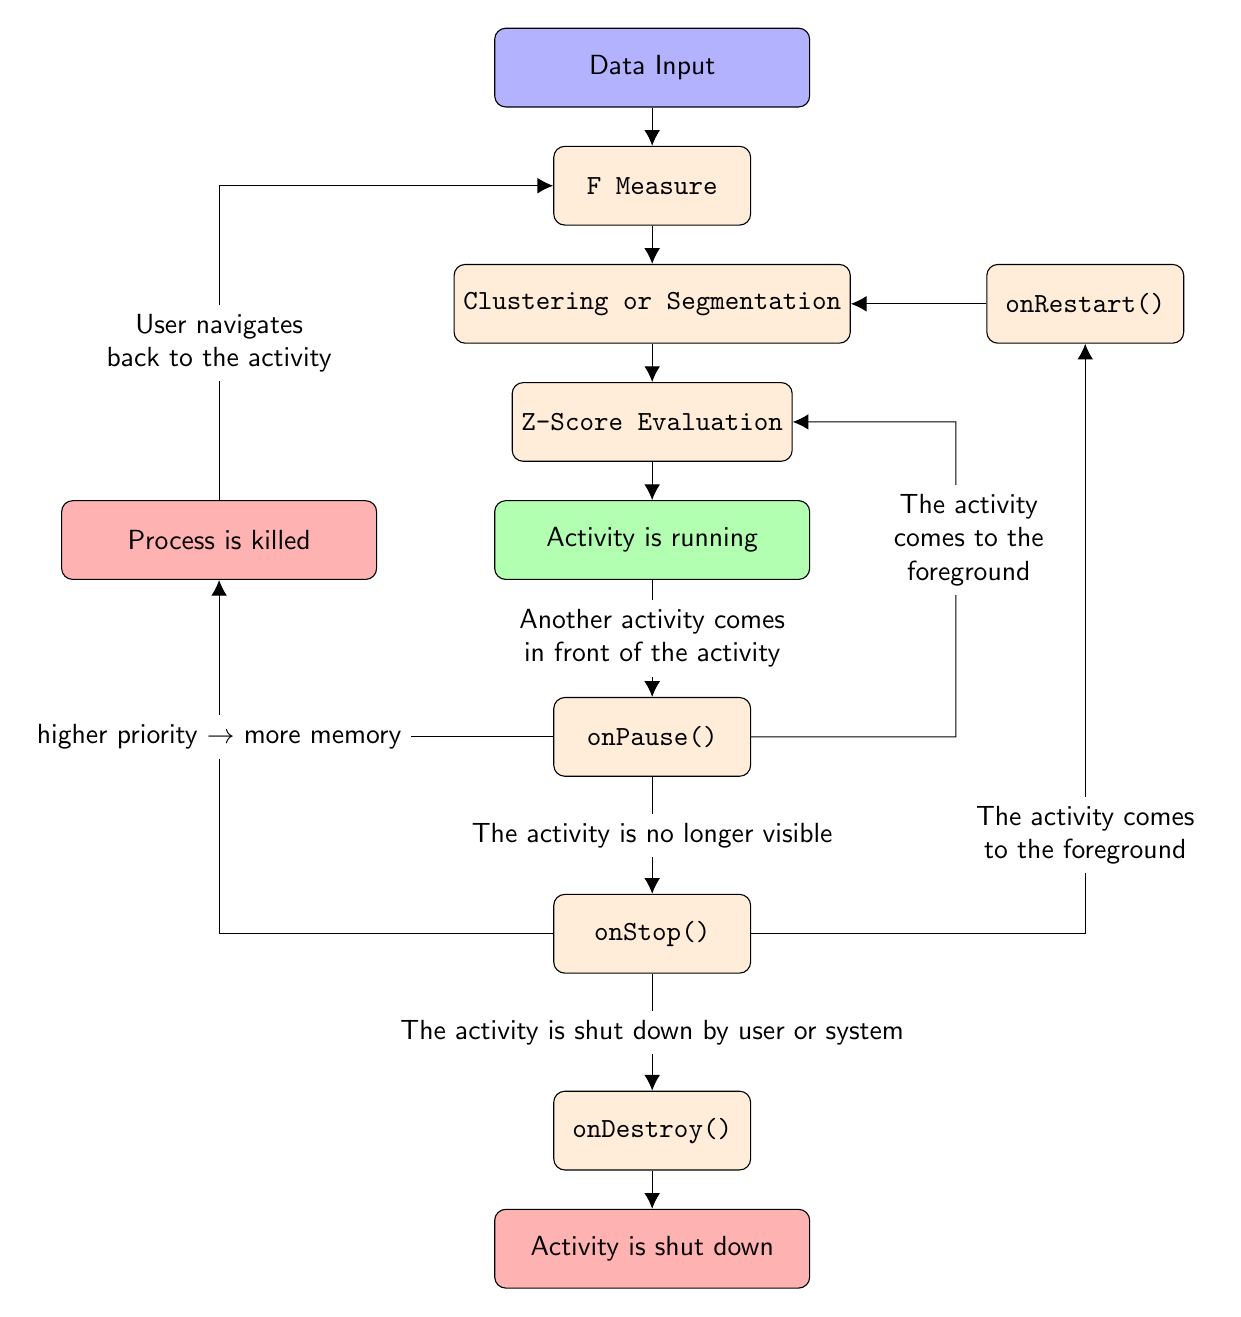
\begin{tikzpicture}[node distance=1.5cm,
    every node/.style={fill=white, font=\sffamily}, align=center]
  % Specification of nodes (position, etc.)
  \node (start)             [activityStarts]              {Data Input};
  \node (onCreateBlock)     [process, below of=start]          {F Measure};
  \node (onStartBlock)      [process, below of=onCreateBlock]   {Clustering or Segmentation};
  \node (onResumeBlock)     [process, below of=onStartBlock]   {Z-Score Evaluation};
  \node (activityRuns)      [activityRuns, below of=onResumeBlock]
                                                      {Activity is running};
  \node (onPauseBlock)      [process, below of=activityRuns, yshift=-1cm]
                                                                {onPause()};
  \node (onStopBlock)       [process, below of=onPauseBlock, yshift=-1cm]
                                                                 {onStop()};
  \node (onDestroyBlock)    [process, below of=onStopBlock, yshift=-1cm] 
                                                              {onDestroy()};
  \node (onRestartBlock)    [process, right of=onStartBlock, xshift=4cm]
                                                              {onRestart()};
  \node (ActivityEnds)      [startstop, left of=activityRuns, xshift=-4cm]
                                                        {Process is killed};
  \node (ActivityDestroyed) [startstop, below of=onDestroyBlock]
                                                    {Activity is shut down};     
  % Specification of lines between nodes specified above
  % with aditional nodes for description 
  \draw[->]             (start) -- (onCreateBlock);
  \draw[->]     (onCreateBlock) -- (onStartBlock);
  \draw[->]      (onStartBlock) -- (onResumeBlock);
  \draw[->]     (onResumeBlock) -- (activityRuns);
  \draw[->]      (activityRuns) -- node[text width=4cm]
                                   {Another activity comes in
                                    front of the activity} (onPauseBlock);
  \draw[->]      (onPauseBlock) -- node {The activity is no longer visible}
                                   (onStopBlock);
  \draw[->]       (onStopBlock) -- node {The activity is shut down by
                                   user or system} (onDestroyBlock);
  \draw[->]    (onRestartBlock) -- (onStartBlock);
  \draw[->]       (onStopBlock) -| node[yshift=1.25cm, text width=3cm]
                                   {The activity comes to the foreground}
                                   (onRestartBlock);
  \draw[->]    (onDestroyBlock) -- (ActivityDestroyed);
  \draw[->]      (onPauseBlock) -| node(priorityXMemory)
                                   {higher priority $\rightarrow$ more memory}
                                   (ActivityEnds);
  \draw           (onStopBlock) -| (priorityXMemory);
  \draw[->]     (ActivityEnds)  |- node [yshift=-2cm, text width=3.1cm]
                                    {User navigates back to the activity}
                                    (onCreateBlock);
  \draw[->] (onPauseBlock.east) -- ++(2.6,0) -- ++(0,2) -- ++(0,2) --                
     node[xshift=1.2cm,yshift=-1.5cm, text width=2.5cm]
     {The activity comes to the foreground}(onResumeBlock.east);
  \end{tikzpicture}

\newpage
\section{Conclusion}

\newpage

\part{Conclusion}

\clearpage

\newpage

\begin{thebibliography}{}

\bibitem{WMG} 
Wei M, Gibbons LW, Mitchell TL \textit{et al}. (1999) The Association between cardiorespiratory fitness and impaired fasting glucose and type 2 diabetes mellitus in men. \textit{Ann Intern Med} \textbf{130}, 427-34.

\bibitem{DEFD}
Jr., W. C. S. (2017, January 26). Definition of Diabetes mellitus. Retrieved November 17, 2019, from https://www.rxlist.com/script/main/art.asp?articlekey=2974.

\bibitem{DBML}
Zou, Q., Qu, K., Luo, Y., Yin, D., Ju, Y.,\& Tang, H. (2018, November 6). Predicting Diabetes Mellitus With Machine Learning Techniques. Retrieved November 17, 2019, from https://www.ncbi.nlm.nih.gov/pmc/articles/PMC6232260/.

\end{thebibliography}
\end{document}